\specialchapter{完备化下的不变性}

\begin{enumerate}
\def\labelenumi{(\alph{enumi})}
\tightlist
\item
  设 A 是一个环，m 是 A 的一个异于 A 的理想。赋予 A 以 m-进拓扑，并以 \(\hat{A}\) 表示其 Hausdorff 完备化。
\end{enumerate}

A 为 Hausdorff 环

是

A 为 Noether 环

是（III, § 3, 命题 8）

A 为局部环

是（III, § 2, 命题 19）

A 为半局部环

是（III, § 2, 命题 19 的推论）

A 为 Zariski 环

是（III, § 3, 命题 8）

\textbf{\(\hat{\mathbf{A}}\)}\par

\begin{enumerate}
\def\labelenumi{(\alph{enumi})}
\setcounter{enumi}{1}
\tightlist
\item
  现在设 \(\mathbf{A}\) 是局部 Noether 环，且 \(\mathfrak{m}\) 是其极大理想。
\end{enumerate}

A 为整环

A 为整闭整环

A 为离散赋值环

A 为约化环

\textbf{\(\hat{\mathbf{A}}\)}\par

否（III, § 3, 习题 15 (b)）

对优良环是（1）

%\pandocbounded{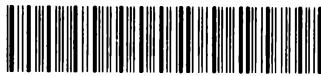
\includegraphics[keepaspectratio]{images/part004_82ba3e9c.jpg}}\\

